\chapter{Implementation and Evaluation}
\label{chap:implemeval}
\textit{\initial{I}n this chapter, we will give some details of implementation, the operating systems we used and the development tools we used, then we will present the evaluation of our solution and comparing our results with the actual solutions presented in this document. The plan of this chapter is as follows : 
}

\minitoc

\newpage
\section{Implementation}

\subsection{The hypervisor}

In order to implement our solution, we had to modify a hypervisor in order to take into account the new design and scheduling algorithms. Since our work is based on the Xen architecture with its privileged domain, we used this latter to implement our solution. Let's note that, our solution is not only specific to Xen but two all hypervisors whose architecture is based on a privileged guest whose role is to execute a number of tasks on behalf of some other guests. 

\textbf{Xen} is a hypervisor written in \textbf{C}, \textbf{Assembly language} and \textbf{Python}. Its source code is composed of about $5000$ files containing more than a million lines of code. To date, Xen is now at version \textbf{4.9} but for stability issues, we worked on its \textbf{4.8} version.

\subsection{The guest \acrshort{os}}
It is important to choose an \acrshort{os} to work on, since the \glspl{dd} code and the \glspl{interrupt} handlers depend on the \acrshort{os}. In this work, we chose \textbf{Linux} for: 

\begin{itemize}
    \item its \glspl{ops} nature which permits us to modify the source code,
    \item its large community of developers, which is active both in native or virtualized domain,
    \item its ability to integrate paravirtualization offered by \textbf{Xen}.
\end{itemize}

The Linux \glspl{kernel} is written in \textbf{C} and \textbf{Assembler}. The source code of Linux is composed of about 14000 files, distributed in about 1000 folders containing about 6 million lines of code. To date, Linux is now at version \textbf{4.12.9} but for compatibility issues with our Xen version, we worked with version \textbf{4.9}.

\subsection{Development tool}
\subsubsection{The compiler}
To compile the Linux \glspl{kernel}, the compiler \textbf{\acrshort{gnu} Compiler Collection (GCC)} must be used. GCC is a set of compilers created by the project \acrshort{gnu}. GCC is a free software enabling compilation of many languages such as C, C++, Objective-C, Java, Ada, and Fortran. In order to use it, we need the tool \textbf{make} to call the GCC compiler. We used the most recent version to date, \textbf{4.2}.
\subsubsection{The editor}

When working on a project containing millions of lines of code such as Linux or Xen, it is important to use an integrated development environment (IDE). However, the disadvantage of IDEs is that they must use their compiler, which is not obvious when programming in the kernel. We opted for the \textbf{Vim editor} and the \textbf{Cscope navigation tool}. Csope is a Linux tool for navigation and exploration of symbols, definitions of symbols, directory structures, and others. It is an integrated tool in Vim. Initially built to work with C code, it currently supports C ++ and Java. During this work, we used the most recent version to date, \textbf{8.0}.

\section{Evaluation}

In order to evaluate our solution, we established a set of synthetic benchmarks to verify that our solution met the objectives for which it was designed and to verify if it performed better than the native implementation. In the section that follows, we will present the different benchmarks we used, their evaluation metrics, the experimental setup and the results obtained comparing it with native solutions. 

\subsection{Benchmark 1: Load generated on the dom0 due to domUs activities}

This synthetic benchmark will permit us to evaluate if our solution, isolates completely a virtual machine preventing the latter to disturb other activities (other domU applications and dom0 administrative tasks) due to the charge generated on the dom0. Here the main metric is the \textbf{load generated} on the dom0 \acrshort{vcpu}.

\subsubsection{Experimental Setup}

The experiment was conducted on a physical computer with the following characteristics : 

\begin{itemize}
    \item 56 processors, 2,5 GHz Intel Xeon,
    \item 40 \acrshort{gb} memory,
    \item Xen 4.8 on Ubuntu 12.04 Linux Kernel 4.9.
\end{itemize}

Here we configured the dom0 to have 2 \acrshort{vcpu} on the main container and 2 \acrshort{gb} main memory. We then increased the number of Domus executing an \acrshort{io} intensive benchmark Iozone and we measured the load generated on the 2 \acrshort{vcpu}. We will then compare with the native solution if the dom0 was configured with 2 \acrshort{vcpu} and 2 \acrshort{gb} main memory.

\subsubsection{Experimental Results}

We can observe on Figure \ref{fig:eval1} that, in the native implementation, the load on the \acrshort{vcpu} increases as the number of Domus increases which can be a cause of performance unpredictability. On the other hand, with our design, the load generated on the 2 \acrshort{vcpu} is nearly constant and does not come from the Domus but from the tasks from group $T_o, T_1 , T_2$.

\subsection{Benchmark 2: Migration time under high load conditions}

This synthetic benchmark will permit us to evaluate if our solution, carries out domU administrative tasks independently on the load on its main container resources. Here the main metric is \textbf{migration time}. 

\subsubsection{Experimental Setup}

The experiment was conducted between 2 physical computers with the following characteristics : 

\begin{itemize}
    \item 8 processors and 4 processors,
    \item 16 \acrshort{gb} memory and 8 \acrshort{gb} memory,
    \item Xen 4.8 on Ubuntu 12.04 Linux Kernel 4.9 on each ,
    \item and linked over a Cisco Catalyst 2960G-24TC-L-Switch.
\end{itemize}

Here the dom0 was configured as in benchmark 1, and the domU to migrate was executing a script whose role was to make random memory accesses in order to simulate memory intensive activities. The migration time was taken and the load on the dom0 main container \acrshort{vcpu} increased.

\subsubsection{Experimental Results}

As shown on Figure \ref{fig:eval2}, with the native implementation, the migration time increases as the load increases, compared to our solution where the migration is nearly constant, due to the fact that the migration task is taken in charge by the secondary containers which are scheduled on the virtual machine resources.

\subsection{Benchmark 3: \acrshort{io} performance as a result of locality}
This synthetic benchmark allows us to evaluate our solution, from a local point of view. Here we  compare the performance obtained when a domU guest executing Iozone benchmark and its resources are distant to those of the dom0. We also measure \textbf{memory bandwidth} for the two approaches, the native implementation, and our design. 

\subsubsection{Experimental Setup}
The experiment was conducted on a physical machine with the following characteristics : 

\begin{itemize}
    \item 8 processors 1,70 GHz Intel Xeon,
    \item 16 \acrshort{gb} memory, 
    \item Xen 4.8 on Ubuntu 12.04 Linux Kernel 4.9 on each.
\end{itemize}

The dom0 was configured as in benchmark 1, and the domU hosts an Iozone benchmark and the metrics were plotted.


\subsubsection{Experimental Results}
As shown on Figure \ref{fig:eval3}, the native implementation bandwidth is lesser than our design bandwidth, due to the fact that, the processes of the dom0 in charge of the domU \acrshort{io} requests are co-located with the domU resources, hence avoiding remote accesses.

\subsection{Benchmark 4: Migration time as a result to locality}

The same principle as for benchmark 3, the only difference is that the metric here is the domU migration time.

\subsubsection{Experimental Setup}
The experiment was conducted on the same conditions as Benchmark 2. Here the domU resources located is placed so that the dom0 resources should be distant to this domain and we launch the domU migration. 

\subsubsection{Experiment Results}

As shown on figure \ref{fig:eval4}, the native implementation migration time is greater than our solution, due to the fact that the process in charge of the migration was co-located with the domU to migrate, hence avoiding remote accesses. 

\section{Review}

These series of benchmarks were realized in order to compare our solution to the native solution over the objectives defined in the introduction. The results obtained in those benchmarks enabled us to conclude that our solution gives a better performance than the native solutions and it meets the objectives for which it was designed. Our solution gives better execution times than native implementations and the execution time is independent of the domUs activities intensity which enables a better billing of the domUs activities. 


\begin{figure}[!h]
\begin{minipage}[b]{.5\linewidth}
\centering 
  \begin{tikzpicture}
  \begin{axis}[legend style={at={(0.5,-0.1)},anchor=north},
  title = {Dom0 \acrshort{vcpu} load},
  ymin = 0,
  legend entries = {Native implementation load (\%),Our solution (\%)}]
  \addplot table {chapters/chapter06/data/expe6.dat};
  \addplot table {chapters/chapter06/data/expe61.dat};
  \end{axis}
  \end{tikzpicture}
\subcaption{Dom0 vcpu load against \# domU guest}
\label{fig:eval1}
\end{minipage}
\begin{minipage}[b]{.5\linewidth}
\centering 
  \begin{tikzpicture}
  \begin{axis}[legend style={at={(0.5,-0.1)},anchor=north},
  title = {domU Migration time},
  ymin = 0,
  legend entries = {Native implementation time (s),Our solution time (s)}]
  \addplot table {chapters/chapter06/data/expe7.dat};
  \addplot table {chapters/chapter06/data/expe71.dat};
  \end{axis}
  \end{tikzpicture}
\subcaption{Migration time against dom0 \acrshort{vcpu} load}
\label{fig:eval2}
\end{minipage}
\caption{First group results}
\end{figure}

\begin{figure}[!h]
    \begin{minipage}[b]{.5\linewidth}
        \centering
        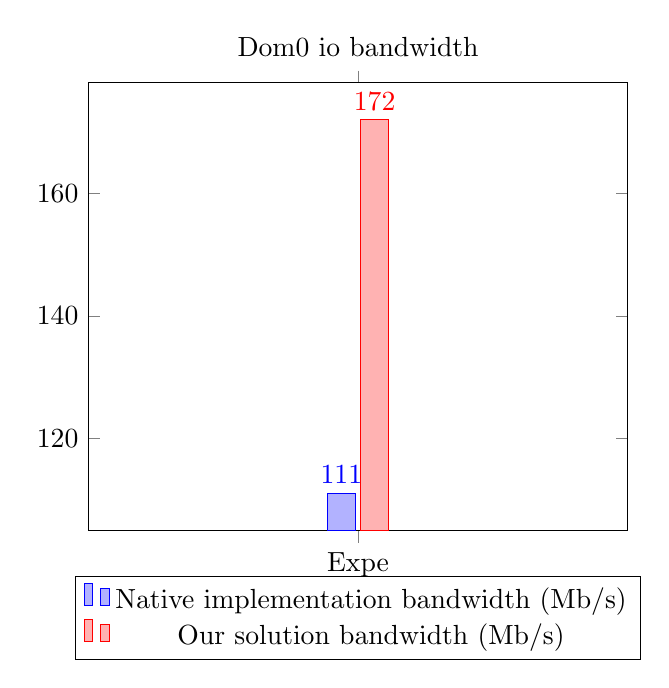
\begin{tikzpicture}
        \begin{axis}[ybar,legend style={at={(0.5,-0.1)},anchor=north},
            symbolic x coords = {Expe},
                   nodes near coords,
                   xtick = data,
                   legend entries = {Native implementation bandwidth (Mb/s),Our solution bandwidth (Mb/s)},
          title = {Dom0 \acrshort{io} bandwidth}]

            \addplot plot coordinates {(Expe,111)};    
            \addplot plot coordinates {(Expe,172) };
          
          \end{axis}
          \end{tikzpicture}
        \subcaption{domU bandwidth against the locality}
        \label{fig:eval3}
    \end{minipage}
    \begin{minipage}[b]{.5\linewidth}
        \centering
        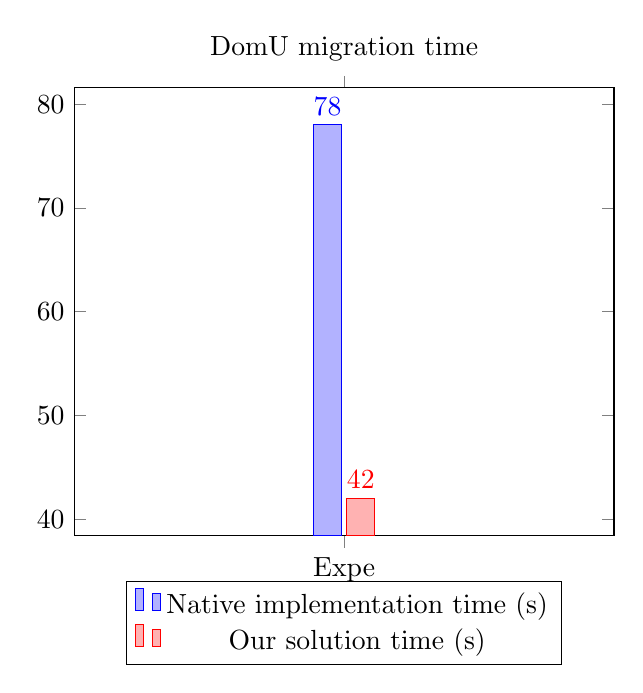
\begin{tikzpicture}
        \begin{axis}[ybar,legend style={at={(0.5,-0.1)},anchor=north},
            symbolic x coords = {Expe},
            xtick = data,
            nodes near coords,
             legend entries = {Native implementation time (s),Our solution time (s)},
          title = {DomU migration time}]
          \addplot plot coordinates {(Expe,78)};
        \addplot plot coordinates {(Expe,42)};
          
          \end{axis}
          \end{tikzpicture}
        \subcaption{domU migration time against the locality}
        \label{fig:eval4}
    \end{minipage}
\caption{Second group results}
\end{figure}
